\documentclass[12pt]{article}
\usepackage[margin=2.5cm]{geometry}
\usepackage{enumerate}
\usepackage{amsfonts}
\usepackage{amsmath}
\usepackage{fancyhdr}
\usepackage{amsmath}
\usepackage{amssymb}
\usepackage{amsthm}
\usepackage{mdframed}
\usepackage{graphicx}
\usepackage{subcaption}
\usepackage{adjustbox}
\usepackage{listings}
\usepackage{xcolor}
\usepackage{booktabs}
\usepackage[utf]{kotex}
\usepackage{hyperref}

\definecolor{codegreen}{rgb}{0,0.6,0}
\definecolor{codegray}{rgb}{0.5,0.5,0.5}
\definecolor{codepurple}{rgb}{0.58,0,0.82}
\definecolor{backcolour}{rgb}{0.95,0.95,0.92}

\lstdefinestyle{mystyle}{
    backgroundcolor=\color{backcolour},
    commentstyle=\color{codegreen},
    keywordstyle=\color{magenta},
    numberstyle=\tiny\color{codegray},
    stringstyle=\color{codepurple},
    basicstyle=\ttfamily\footnotesize,
    breakatwhitespace=false,
    breaklines=true,
    captionpos=b,
    keepspaces=true,
    numbers=left,
    numbersep=5pt,
    showspaces=false,
    showstringspaces=false,
    showtabs=false,
    tabsize=1
}

\lstset{style=mystyle}

\pagestyle{fancy}
\renewcommand{\headrulewidth}{0.4pt}
\lhead{CSC 209}
\rhead{Review 6 Solution}

\begin{document}
\title{CSC 209 Review 6 Solution}
\maketitle

\bigskip

\section{Exercises}

\begin{enumerate}[1.]
    \item

    I need to write which of the supplied function calls don't work and explain why.

    \bigskip

    \begin{itemize}
        \item \texttt{b)} String format in \texttt{printf} expects character constant, but string literal is used
        \item \texttt{c)} String format in \texttt{printf} expects string but character constrant is used
        \item \texttt{e)} The first argument in \texttt{printf} expects pointer but character constrant (an integer) is used isntead
        \item \texttt{h)} The first argument in \texttt{putchar} expects a character, but string literal (a pointer to character) is used
        \item \texttt{i)} The first argument in \texttt{puts} expects a pointer to character, but character constant (an integer) is used
    \end{itemize}

    \underline{\textbf{Notes}}

    \begin{itemize}
        \item \textbf{putchar}

        \begin{itemize}
            \item \textbf{Syntax:} \texttt{int putchar(int char)}
            \item Writes a character (an unsigned char) specified by the argument char to stdout.
            \item Does not append a new line to the output
            \item Is similar to printf but for character
        \end{itemize}

        \item \textbf{puts}

        \begin{itemize}
            \item \textbf{Syntax:} \texttt{int puts(const char *str)}
            \item Writes a string to stdout up to but not including the null character
            \item Appends a newline character to the output.
            \item Is similar to printf but for string
        \end{itemize}

        \item \textbf{Character Constant}

        \begin{itemize}
            \item \textbf{Syntax:} \texttt{' ... '}
            \item Is represented by an \underline{integer}
        \end{itemize}

        \item \textbf{String Literal}
        \begin{itemize}
            \item \textbf{Syntax:} \texttt{" ... "}
            \item Has a sequence of characters inside
            \item Ends with \texttt{$\backslash$0}
            \item Is represented by a \underline{pointer}

            \bigskip

            \underline{\textbf{Example}}

            \bigskip

            "When you come to a fork in the road, take it"
        \end{itemize}

        \item \textbf{Escape Squences in String Literal}

        \begin{itemize}
            \item A common example is `\texttt{$\backslash$n}'

            \begin{itemize}
                \item causes the cursor to advance to the next line
            \end{itemize}
        \end{itemize}
    \end{itemize}

    \item

    First, I need to write which of the provided function calls are legal, and write the output
    produced

    \bigskip

    The solution to the first part is:

    \begin{itemize}
        \item \texttt{b)} [output: a]
        \item \texttt{c)} [output: abc]
    \end{itemize}

    \bigskip

    Second, I need to write which of the following function calls are illegal, and explain why.

    \bigskip

    The solution to the second part is:

    \begin{itemize}
        \item \texttt{a)} \texttt{purchar} expects a character constant (an integer) but a value of type pointer to \texttt{char} is used
        \item \texttt{d)} \texttt{puts} expects a variable of type pointer to \texttt{char}, but a variable of type pointer to \texttt{char} is used
    \end{itemize}

    \item

    I need to write the values of \texttt{i}, \texttt{j}, \texttt{k} in the function

    \bigskip

    \texttt{scanf("\%d\%s\%d", \&i, s, \&j)}

    \bigskip

    if the user enters \texttt{12abc34 56def78}.

    \bigskip

    The solution to this problem is:

    \begin{itemize}
        \item \texttt{i} - \texttt{12}
        \item \texttt{j} - \texttt{abc34 }
        \item \texttt{k} - \texttt{56}
    \end{itemize}

    \item

    I need to modify the following \texttt{read\_line} function in the following ways:

    \begin{center}
    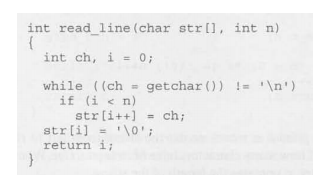
\includegraphics[width=0.7\linewidth]{images/review_6_solution_1.png}
    \end{center}

    \begin{enumerate}[a)]
        \item Have it skip white space beore beginning to store input characters
        \item Have it stop reading at the first white-space character
        \item Have it stop reading at the first new-line character, then store the new-line character in the string
        \item Have it leave behind characters that it doesn't have room to store
    \end{enumerate}

    \bigskip

    The solution to this problem is:

    \begin{enumerate}[a)]
        \item

\begin{lstlisting}[language=c]
    #include <ctype.h>
    #include <stdbool.h>

    ...

    int read_line(char str[], int n)
    {
        int ch, i = 0;
        bool non_space_char_exists = false;

        while ((ch = getchar()) != '\n')
            if (isspace(ch) && non_space_char_exists){
                continue;
            }

            if (i < n)
                str[i++] = ch;
                non_space_char_exists = true;
        str[i] = '\0';
        return i;
    }
\end{lstlisting}

        \item

\begin{lstlisting}[language=c]
    #include <ctype.h>

    ...

    int read_line(char str[], int n)
    {
        int ch, i = 0;

        while ((ch = getchar()) != '\n')
            if (isspace(ch)){
                break;
            }

            if (i < n)
                str[i++] = ch;
        str[i] = '\0';
        return i;
    }
\end{lstlisting}

        \item

\begin{lstlisting}[language=c]
    #include <ctype.h>

    ...

    int read_line(char str[], int n)
    {
        int ch, i = 0;

        while ((ch = getchar()) != '\n')
            if (ch == '\n'){
                break;
            }

            if (i < n)
                str[i++] = ch;

        str[i] = '\n';
        str[i+1] = '\0';
        return i;
    }
\end{lstlisting}

        \item

\begin{lstlisting}[language=c]
    #include <ctype.h>

    ...

    int read_line(char str[], int n)
    {
        int ch, i = 0;
        int n = strlen(str) + 1;

        do {
            ch = getchar();

            if (!ch) {
                break;
            }

            str[i++] = ch;

        } while (i < (n - 1));

        str[i] = '\0';
        return i;
    }
\end{lstlisting}


    \end{enumerate}

    \bigskip

    \begin{mdframed}
    \underline{\textbf{Correct Solution}}

    \bigskip

    \begin{itemize}

        \item \texttt{c)}

\begin{lstlisting}[language=c]
    #include <ctype.h>

    ...

    int read_line(char str[], int n)
    {
        int ch, i = 0;

        do {
            ch = getchar()

            if (ch == '\n'){
                break;
            }

            if (i < n)
                str[i++] = ch;

        } while (ch !== '\n');

        str[i] = '\0';
        return i;
    }
\end{lstlisting}

        \item \texttt{d)}

\begin{lstlisting}[language=c]
    #include <ctype.h>

    ...

    int read_line(char str[], int n)
    {
        int ch, i = 0;
        int n = strlen(str) + 1;

        do {
            ch = getchar();

            if (ch == '\n') {
                break;
            }

            str[i++] = ch;

        } while (i < (n - 1));

        str[i] = '\0';
        return i;
    }
\end{lstlisting}


    \end{itemize}


    \end{mdframed}

    \bigskip

    \underline{\textbf{Notes}}

    \begin{itemize}
        \item Learned that \texttt{getchar()} always ends with \texttt{$\backslash$n}
    \end{itemize}

    \item

    \begin{enumerate}[a)]
        \item

        I need to write a function named \texttt{capitalize} that capitalizes all
        letters in its argument.

        \bigskip

        The requirement for this function is:

        \bigskip

        \begin{itemize}
            \item Array subscripting must be used to access each character in string
        \end{itemize}

        \bigskip

        The solution to this problem is:

        \bigskip

\begin{lstlisting}[language=c]
    #include <ctype.h> // toupper

    void capitalize(char *s)
    {

        for (int i = 0; s[i] != '\0'; i++) {
            s[i] = toupper(s[i]);
        }
    }
\end{lstlisting}

        \bigskip

        \underline{\textbf{Notes}}

        \begin{itemize}
            \item \textbf{Accessing the Characters in a String}

            \begin{enumerate}[1.]
                \item Using array subscripting

                \bigskip

                \underline{\textbf{Example}}

                \bigskip

                \begin{center}
                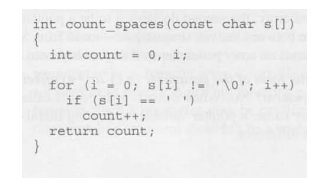
\includegraphics[width=0.7\linewidth]{images/review_6_solution_2.png}
                \end{center}

                \bigskip

                \item Using pointer

                \bigskip

                \underline{\textbf{Example}}

                \bigskip

                \begin{center}
                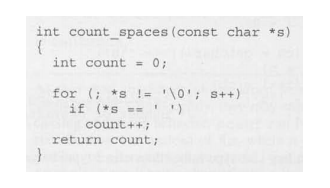
\includegraphics[width=0.7\linewidth]{images/review_6_solution_3.png}
                \end{center}

                \bigskip

            \end{enumerate}
        \end{itemize}

        \item

        I need to write a function named \texttt{capitalize} that capitalizes all
        letters in its argument.

        \bigskip

        The requirement for this function is:

        \bigskip

        \begin{itemize}
            \item pointer must be used to access each character in string
        \end{itemize}

        \bigskip

        The solution to this problem is:

        \bigskip

\begin{lstlisting}[language=c]
    #include <ctype.h> // toupper

    void capitalize(char *s)
    {
        char *p = s;
        while (*p != '\0') {
            *p = toupper(*p);
            p++;
        }
    }
\end{lstlisting}

    \end{enumerate}

    \item

    I need to write a function \texttt{censor} that modifies a string by replacing
    every occurence of \texttt{foo} with \texttt{***}.

    \bigskip

    The additional requirement of this function are:

    \begin{itemize}
        \item I need to make the function as short as possible without sacrificing
        clarity.
    \end{itemize}

    \bigskip

    The solution to this problem is:

    \bigskip

\begin{lstlisting}[language=c]
#include <string.h> \\ strlen

void censor(char s[]) {
    char *p;

    if (strlen(s) < 3) {
        return;
    }

    for (p = &s[2]; p < s + strlen(s); p++) {
        if (tolower(*p) == 'o' &&
            tolower(*(p-1)) == 'o' &&
            tolower(*(p-2)) == 'f') {

            *p = '*';
            *(p-1) = '*';
            *(p-2) = '*';
        }
    }

}
\end{lstlisting}

    \bigskip


    \begin{mdframed}
    \underline{\textbf{Correct Solution}}

    \bigskip

    \begin{lstlisting}[language=c]
        #include <string.h> \\ strlen

        void censor(char s[]) {
            if (strlen(s) < 3) {
                return;
            }

            for (char *p = &s[2]; *p != '\0'; p++) {
                if (tolower(*p) == 'o' &&
                    tolower(*(p-1)) == 'o' &&
                    tolower(*(p-2)) == 'f') {

                    *p = *(p-1) = *(p-2) = '*';
                }
            }

        }
        \end{lstlisting}

    \end{mdframed}

    \item

    I need to identify from the provided statements that which is not equivalent to others.

    \bigskip

    The solution to this problem is:

    \begin{itemize}
        \item \texttt{d)} All of the other statments are about making \texttt{str} null or empty.
    \end{itemize}

    \bigskip

    \underline{\textbf{Notes}}

    \begin{itemize}
        \item \texttt{*str = 0} makes pointer \texttt{NULL}
        \item \textbf{strcpy}

        \begin{itemize}
            \item \textbf{Syntax:} \texttt{char *strcpy (char *s1, const char *s2)}
            \item Copies string \texttt{s2} to the string \texttt{s1}
        \end{itemize}

        \item \textbf{strcat}

        \begin{itemize}
            \item \textbf{Syntax:} \texttt{char *strcat(char *s1, const char *s2)}
            \item appends the contents of the string \texttt{s2} to the end of the string \texttt{s1}
        \end{itemize}

        \bigskip

        \underline{\textbf{Example}}

        \bigskip

        \begin{center}
        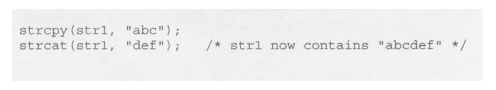
\includegraphics[width=0.8\linewidth]{images/review_6_solution_4.png}
        \end{center}
    \end{itemize}

    \item

    I need to write the value of the string \texttt{str} after the following execution
    of statements

    \begin{center}
    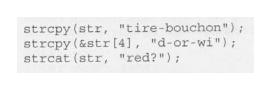
\includegraphics[width=0.5\linewidth]{images/review_6_solution_5.png}
    \end{center}

    The solution to this problem is: \texttt{tired-or-winred?}

    \bigskip

    \begin{mdframed}
    \underline{\textbf{Correct Solution}}

    \bigskip

    The solution to this problem is: \texttt{tired-or-wired?}
    \end{mdframed}

    \bigskip

    \underline{\textbf{Notes}}

    \bigskip

    \begin{itemize}
        \item \texttt{strcpy} always copies \underline{upto} the first null character.

        \begin{itemize}
            \item The pointer stops and points at the first null character after \texttt{strcpy}
        \end{itemize}
    \end{itemize}

    \item

    I need to write the value of the string \texttt{s1} after the executing the provided statements:

    \bigskip

    The solution to this problem is: \texttt{computers}

    \bigskip

    \begin{mdframed}
    \underline{\textbf{Correct Solution}}

    \bigskip

    The solution to this problem is: \texttt{computers\color{red}$\backslash$0\color{black}}

    \end{mdframed}


    \bigskip

    \underline{\textbf{Notes}}

    \begin{itemize}
        \item \textbf{strcmp}

        \begin{itemize}
            \item \textbf{Syntax:} \texttt{int strcmp(const char *s1, const char *s2)}

            \begin{itemize}
                \item Compares string \texttt{s1} and \texttt{s2}
                \item Returns

                \begin{itemize}
                    \item \texttt{0} - if \texttt{s1} and \texttt{s2} are identical
                    \item \texttt{$>$0} - if ASCII value of first unmatched character in \texttt{s1} is greater than \texttt{s2}
                    \item \texttt{$<$0} - if ASCII value of first unmatched character in \texttt{s1} is less than \texttt{s2}
                \end{itemize}
            \end{itemize}
        \end{itemize}
    \end{itemize}

    \item

    I need to write what's wrong with the provided function.

    \bigskip

    The solution to this problem is that the pointer \texttt{*q} hasn't
    allocated memory, and because of that, the function call \texttt{strcpy(q,p)} would result in segmentation fault.

    \item

    Here I need to modify \texttt{strcmp} function to use pointer arithmetic.

    \bigskip

    The solution to this problem is:

    \bigskip

\begin{lstlisting}[language=c]
    int strcmp (char *s, char *t) {
        char *p = s, *q = t;

        while (*p == *q) {
            if (*p == '\0') {
                return 0;
            }
            p++;
            q++;
        }

        return *p - *q;
    }
\end{lstlisting}

    \bigskip

    \item

    I need to write the following function

    \bigskip

    \texttt{void get\_extension(const char *file\_name, char *extension)}

    \bigskip

    satisfying the following requirements:

    \begin{itemize}
        \item If the file name doesn't have an extension, empty string should be stored instead
        \item \texttt{get\_extension} should be kept as simple as possible by using \texttt{strlen} and \texttt{strcpy}
    \end{itemize}

    \bigskip

    The solution to this problem is:

    \bigskip

\begin{lstlisting}[language=c]
    void get_extension(const char *file_name, char *extension) {
        int i = strlen(file_name) - 1;

        for (; i >= 0; i--) {
            if (*(file_name+i) == '.') {
                break;
            }
        }
        strcpy(extension, file_name + (i+1));
    }
\end{lstlisting}

    \item

    I need to write the following function

    \bigskip

    \texttt{void build\_index\_url (const char *domain, char *index\_url);}

    \bigskip

    satisfying the following requirements:

    \begin{itemize}
        \item \texttt{build\_index\_url} should add "http://www." to the beginning of the string
        \item \texttt{build\_index\_url} should add "/index.html" to the end of the string
        \item \texttt{build\_index\_url} should store the result in \texttt{index\_url}
        \item \texttt{build\_index\_url} should be kept as simple as possible by using \texttt{strcat} and \texttt{strcpy}
    \end{itemize}

    \bigskip

    The solution to this problem is:

    \bigskip


\begin{lstlisting}[language=c]
    void build_index_url (const char *domain, char *index_url) {
        strcat(index_url, "http://www.");
        strcat(index_url, domain);
        strcat(index_url, "/index.html");
    }
\end{lstlisting}

    \item

    I need to write the output of the provided function.

    \bigskip

    The solution to this problem is: \texttt{Grinch}

    \bigskip

\begin{lstlisting}[language=c]

\end{lstlisting}

    \bigskip

    \underline{\textbf{Notes}}

    \bigskip

    \begin{itemize}
        \item \texttt{--*p} means decrement \texttt{*p} first; the value of expression is \texttt{*p} after decrement
        \item Idioms are good to know. It's used by a lot of C programmers.
        \item \textbf{String Idioms - Searching for the end of string}

        \begin{itemize}
            \item The following function \texttt{strlen} are equal

            \bigskip

            \begin{center}
            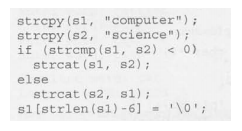
\includegraphics[width=0.9\linewidth]{images/review_6_solution_6.png}
            \end{center}

            \bigskip

            It takes advantage of the fact that the end of string is \texttt{*s = '$\backslash$0' = 0}

        \end{itemize}

        \item \textbf{String Idioms - Copying string}

        \begin{itemize}
            \item The following function \texttt{strlen} are equal

            \bigskip

            \begin{center}
            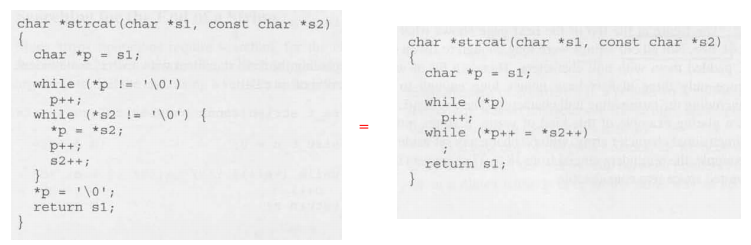
\includegraphics[width=0.9\linewidth]{images/review_6_solution_7.png}
            \end{center}

            \bigskip

        \end{itemize}
    \end{itemize}

    \item

    \begin{enumerate}[a)]
        \item

        I need to find the value of \texttt{f("abcd","babc")} given the provided function \texttt{f}.

        \bigskip

        The solution to this problem is: \texttt{3}

        \bigskip

        \item

        I need to find the value of \texttt{f("abcd","bcd")} given the provided function \texttt{f}.

        \bigskip

        The solution to this problem is: \texttt{0}

        \bigskip

        \item

        I need to write what value \texttt{f} returns when two strings \texttt{s}
        and \texttt{t} are passed.

        \bigskip

        The answer to this problem is: it returns the number of consequtive characters in \texttt{s} that's also in \texttt{t}.

    \end{enumerate}

    \item

    I need to use the techniques of section 13.6 to condense the function \texttt{count\_spaces}
    in section 13.4

    \bigskip

    The solution to this problem is:

    \bigskip

\begin{lstlisting}[language=c]
int count_spaces(const char s[])
{
    int count = 0;

    do {
        if (*s == ' ') {
            count++;
        }
    } while (*s++);

    return count;
}
\end{lstlisting}

    \item

    I need to write the following function

    \bigskip

    \texttt{bool test\_extension (const char *file\_name, const char *extension)}

    \bigskip

    satisfying the following requiremnts

    \begin{itemize}
        \item \texttt{test\_extension} should return \texttt{true} if the file's extension matches the string
        pointed to by \texttt{extension}.
        \item \texttt{test\_extension} should ignore the case of letters
        \item \texttt{test\_extension} should use ``search for the end of a string'' idiom
        \item \texttt{test\_extension} should use \texttt{toupper} to make the process case-insensitive
    \end{itemize}

    \bigskip

    The solution to this problem is:

    \bigskip

\begin{lstlisting}[language=c]
    bool test_extension (const char *file_name, const char *extension)
    {
        while (*file_name++ != '.')
            ;


        while (toupper(*file_name++) == toupper(*extension++)) {
            if (*file_name == '\0' && *extension == '\0') {
                return true;
            }
        }

        return false;
    }
\end{lstlisting}

    \item

    I need to write the function

    \bigskip

    \texttt{void remove\_filename(char *url)}

    \bigskip

    satisfying the following requirements

    \begin{itemize}
        \item \texttt{remove\_filename} shold modify the string in \texttt{url} by
        removing the file name and the preceding slash

        \bigskip

        \texttt{http://www.knking.com/index.html} $\to$ \texttt{http://www.knking.com/}

        \item \texttt{remove\_filename} should use "search for the end of a string" idiom
    \end{itemize}

    \bigskip

    The solution to this problem is:

    \bigskip

\begin{lstlisting}[language=c]
    void remove_filename(char *url)
    {
        char *p = url;

        while (*p++)
            ;

        while (p-- > url) {
            if (*p == '/') {
                *p = '\0';
                return;
            }
        }
    }
\end{lstlisting}


\end{enumerate}

\bigskip

\section{Programming Exercise}

\begin{enumerate}[1.]
    \item

    I need to write a program that finds the "smallest" and "largest" in a series of
    words.

    \bigskip

    The requirement for this program are:

    \begin{itemize}
        \item The program should ask the user to enter the words
        \item The program should determine which words comes first and last as if the words are listed in dictionary order
        \item The program must stop accepting input when the user enters a four-letter word
        \item Assume program has no word more than 20 letters long
        \item The program should use \texttt{smallest\_word} and \texttt{largest\_word} to keep trak
        of the "smallest" and "largest" words so far.
        \item The program should use \texttt{strcmp} to compare with \texttt{smallest\_word}
        \item The program should also use \texttt{strcmp} to comapre with \texttt{largest\_word}
        \item The program should use \texttt{strlen} to determine when the user entered a four-letter word
    \end{itemize}

    \bigskip

    The solution to this problem is included in file \texttt{question\_19.c}.


    \item

    \begin{enumerate}[a)]
        \item

        I need to improve the \texttt{remind.c} with the following requirements:

        \begin{itemize}
            \item The program should print an error message and ignore a reminder if the corresponding day is negative or larger than 31
            using \texttt{continue} statement
        \end{itemize}

        \bigskip

        The solution to this problem is included in file \texttt{question\_20\_a.c}.
    \end{enumerate}
\end{enumerate}



\end{document}